% SC2000 — Chapter 6: Joint Distributions & Central Limit Theorem
\chapter{Joint Distributions \& the Central Limit Theorem}
\label{ch:joint}

\begin{quote}
\emph{``One variable tells a story; two variables tell the truth.''} Response time and server load, accuracy and training size, height and weight---computing data is multivariate. Joint distributions describe how variables move together, and the Central Limit Theorem explains why averages of many small effects are always Normal.
\end{quote}

\noindent\fbox{\parbox{\dimexpr\linewidth-2\fboxsep-2\fboxrule}{%
\textbf{From zero: pairs of outcomes.} We extend PMF/PDF to two variables, define joint, marginal, and conditional distributions, then build covariance through to the CLT---the most important theorem in statistics.}}
\vspace{0.4em}

\section*{Learning Outcomes}
After this chapter you will be able to:
\begin{enumerate}[label=(L\arabic*)]
    \item write joint, marginal, and conditional PMFs/PDFs and translate between them;
    \item test independence via factorisation and compute $\mathrm{Cov}$, $\rho$;
    \item apply the weak and strong laws of large numbers;
    \item state and use the Central Limit Theorem (CLT) with continuity correction;
    \item recognise when CLT justifies Normal approximations for averages and sums.
\end{enumerate}

% ============================================================
\section{Joint, Marginal, and Conditional Distributions}
\label{sec:joint-def}

\begin{definition}[Joint PMF/PDF] For discrete $(X,Y)$, $p_{X,Y}(x,y)=P(X=x,Y=y)$. For continuous, $f_{X,Y}$ with $P((X,Y)\in A)=\iint_A f_{X,Y}(x,y)\,dx\,dy$. Marginals: $p_X(x)=\sum_y p_{X,Y}(x,y)$ (or $\int f_{X,Y}\,dy$). Conditional: $p_{X\mid Y}(x\mid y)=p_{X,Y}(x,y)/p_Y(y)$.
\end{definition}

\emph{Table intuition:} a joint PMF is a matrix; rows sum to $p_Y$, columns to $p_X$. Conditioning on $Y=y$ picks one row and renormalises.

\begin{figure}[h]
\centering
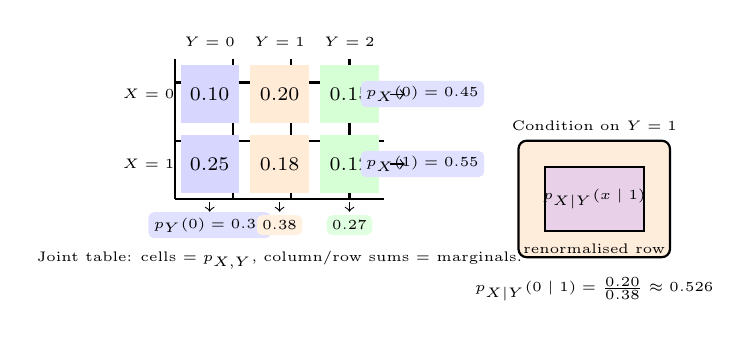
\begin{tikzpicture}[scale=0.74,every node/.style={font=\scriptsize}]
% Joint table as colored grid
\draw[thick] (0,0) grid (3.6,2.4);
% header
\node[font=\tiny\bfseries] at (0.6,2.7) {$Y=0$}; \node[font=\tiny\bfseries] at (1.8,2.7) {$Y=1$}; \node[font=\tiny\bfseries] at (3.0,2.7) {$Y=2$};
\node[font=\tiny\bfseries] at (-0.45,1.8) {$X=0$}; \node[font=\tiny\bfseries] at (-0.45,0.6) {$X=1$};
% cells with probabilities (example)
\foreach \x/\y/\p/\col in {0.6/1.8/0.10/blue,1.8/1.8/0.20/orange,3.0/1.8/0.15/green,0.6/0.6/0.25/blue,1.8/0.6/0.18/orange,3.0/0.6/0.12/green} {
  \fill[\col!16] (\x-0.5,\y-0.5) rectangle (\x+0.5,\y+0.5);
  \node at (\x,\y) {$\p$};
}
% marginals
\node[font=\tiny,fill=blue!12,rounded corners=2pt,inner sep=2pt] at (0.6,-0.45) {$p_Y(0)=0.35$};
\node[font=\tiny,fill=orange!12,rounded corners=2pt,inner sep=2pt] at (1.8,-0.45) {$0.38$};
\node[font=\tiny,fill=green!12,rounded corners=2pt,inner sep=2pt] at (3.0,-0.45) {$0.27$};
\node[font=\tiny,fill=blue!12,rounded corners=2pt,inner sep=2pt] at (4.25,1.8) {$p_X(0)=0.45$};
\node[font=\tiny,fill=blue!12,rounded corners=2pt,inner sep=2pt] at (4.25,0.6) {$p_X(1)=0.55$};
\draw[->,thin] (3.7,1.8)--(3.95,1.8); \draw[->,thin] (3.7,0.6)--(3.95,0.6);
\draw[->,thin] (0.6,-0.05)--(0.6,-0.22); \draw[->,thin] (1.8,-0.05)--(1.8,-0.22); \draw[->,thin] (3.0,-0.05)--(3.0,-0.22);
\node[font=\tiny,align=center] at (1.8,-1.05) {Joint table: cells $=p_{X,Y}$, column/row sums $=$ marginals.};
% Right: conditioning illustration
\begin{scope}[xshift=7.2cm]
\draw[thick,fill=orange!14,rounded corners=3pt] (-1.3,-1.0) rectangle (1.3,1.0);
\node[font=\tiny] at (0,1.25) {Condition on $Y=1$};
\draw[thick,fill=violet!18] (-0.85,-0.55) rectangle (0.85,0.55);
\node[font=\tiny] at (0,0) {$p_{X\mid Y}(x\mid1)$};
\node[font=\tiny,align=center] at (0,-0.85) {renormalised row};
\node[font=\tiny,align=center] at (0,-1.55) {$p_{X\mid Y}(0\mid1)=\frac{0.20}{0.38}\approx0.526$};
\end{scope}
\end{tikzpicture}
\caption{Joint PMF as a table: marginals are row/column sums; conditioning picks a row/column and renormalises.}
\label{fig:joint-table}
\end{figure}

\begin{definition}[Independence] $X,Y$ independent iff $p_{X,Y}(x,y)=p_X(x)p_Y(y)$ (or $f_{X,Y}=f_Xf_Y$) for all $x,y$. Equivalently $F_{X,Y}(x,y)=F_X(x)F_Y(y)$.
\end{definition}

% ============================================================
\section{Covariance and Correlation Revisited}
\label{sec:cov-joint}
For jointly distributed $(X,Y)$ with means $\mu_X,\mu_Y$,
\[
\mathrm{Cov}(X,Y)=\mathbb{E}[(X-\mu_X)(Y-\mu_Y)]=\mathbb{E}[XY]-\mu_X\mu_Y,\qquad
\rho_{X,Y}=\frac{\mathrm{Cov}(X,Y)}{\sigma_X\sigma_Y}\in[-1,1].
\]
Cauchy--Schwarz gives $|\mathrm{Cov}|\le\sigma_X\sigma_Y$. If independent, $\mathrm{Cov}=0$ (but not conversely---see Ch.~5 Ex.~4).

\emph{Computing use:} covariance matrices summarise feature relationships; diagonal $=$ variances, off-diagonal $=$ covariances. PCA diagonalises this matrix.

% ============================================================
\section{Laws of Large Numbers}
\label{sec:lln}

\begin{theorem}[Weak Law of Large Numbers, WLLN] If $X_i$ i.i.d.\ with mean $\mu$ and finite variance, sample mean $\bar X_n=\frac1n\sum_{i=1}^n X_i$ satisfies for every $\varepsilon>0$,
\[
P(|\bar X_n-\mu|\ge\varepsilon)\xrightarrow[n\to\infty]{}0.
\]
Proof via Chebyshev: $P(|\bar X_n-\mu|\ge\varepsilon)\le\mathrm{Var}(\bar X_n)/\varepsilon^2=\sigma^2/(n\varepsilon^2)$.
\end{theorem}

\begin{theorem}[Strong Law, SLLN] Under same conditions, $P(\lim_{n\to\infty}\bar X_n=\mu)=1$ (almost sure convergence).
\end{theorem}

\emph{Meaning:} Monte Carlo works. Averaging many i.i.d.\ simulation runs converges to the true expectation. This justifies empirical estimation throughout computing.

% ============================================================
\section{Central Limit Theorem}
\label{sec:clt}

\begin{theorem}[Central Limit Theorem, Lindeberg--L\'evy] If $X_i$ i.i.d.\ with mean $\mu$ and variance $\sigma^2<\infty$, then
\[
\frac{\sum_{i=1}^n X_i-n\mu}{\sigma\sqrt{n}}=\frac{\bar X_n-\mu}{\sigma/\sqrt{n}}\xrightarrow[d]{}\mathcal{N}(0,1).
\]
That is, for large $n$, $\sum X_i\approx\mathcal{N}(n\mu,n\sigma^2)$ and $\bar X_n\approx\mathcal{N}(\mu,\sigma^2/n)$.
\end{theorem}

Why it matters: \emph{any} sum/average of many small independent effects is approximately Normal, regardless of the underlying distribution (provided variance finite). Measurement errors, aggregated latencies, poll averages, stochastic gradient noise---all Normal by CLT.

\begin{figure}[h]
\centering
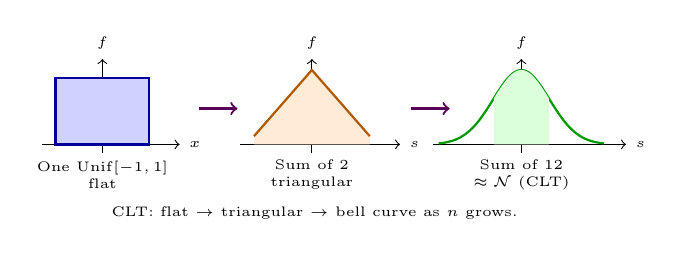
\begin{tikzpicture}[scale=0.70,every node/.style={font=\scriptsize}]
% Three stages: uniform -> sum of 2 -> sum of 12 ~ Normal
\begin{scope}
\draw[->,thin] (-1.1,0)--(1.4,0) node[right,font=\tiny] {$x$};
\draw[->,thin] (0,-0.15)--(0,1.55) node[above,font=\tiny] {$f$};
\fill[blue!18] (-0.85,0) rectangle (0.85,1.2);
\draw[thick,blue!60!black] (-0.85,0) rectangle (0.85,1.2);
\node[font=\tiny,align=center] at (0,-0.55) {One $\mathrm{Unif}[-1,1]$\\flat};
\end{scope}
\begin{scope}[xshift=3.8cm]
\draw[->,thin] (-1.3,0)--(1.6,0) node[right,font=\tiny] {$s$};
\draw[->,thin] (0,-0.15)--(0,1.55) node[above,font=\tiny] {$f$};
\fill[orange!16] (-1.05,0) -- (-1.05,0.15) -- (0,1.35) -- (1.05,0.15) -- (1.05,0) -- cycle;
\draw[thick,orange!70!black] (-1.05,0.15)--(0,1.35)--(1.05,0.15);
\node[font=\tiny,align=center] at (0,-0.55) {Sum of $2$\\triangular};
\end{scope}
\begin{scope}[xshift=7.6cm]
\draw[->,thin] (-1.6,0)--(1.9,0) node[right,font=\tiny] {$s$};
\draw[->,thin] (0,-0.15)--(0,1.55) node[above,font=\tiny] {$f$};
\draw[thick,green!60!black,smooth,domain=-1.5:1.5,samples=60] plot (\x,{1.35*exp(-\x*\x/0.52)});
\fill[green!14] (-0.5,0) -- plot[domain=-0.5:0.5,samples=30] (\x,{1.35*exp(-\x*\x/0.52)}) -- (0.5,0) -- cycle;
\node[font=\tiny,align=center] at (0,-0.55) {Sum of $12$\\$\approx\mathcal{N}$ (CLT)};
\end{scope}
\draw[->,thick,violet!70!black] (1.75,0.65)--(2.45,0.65);
\draw[->,thick,violet!70!black] (5.6,0.65)--(6.3,0.65);
\node[font=\tiny,align=center] at (3.85,-1.25) {CLT: flat $\to$ triangular $\to$ bell curve as $n$ grows.};
\end{tikzpicture}
\caption{CLT in action: summing i.i.d.\ $\mathrm{Uniform}[-1,1]$ variables. One is flat, two is triangular, twelve is already bell-shaped.}
\label{fig:clt-demo}
\end{figure}

\begin{figure}[h]
\centering
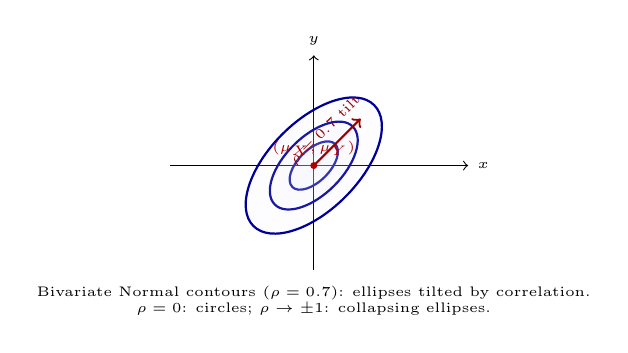
\begin{tikzpicture}[scale=0.70,every node/.style={font=\scriptsize}]
% Bivariate normal contours
\draw[->,thin] (-2.6,0)--(2.8,0) node[right,font=\tiny] {$x$};
\draw[->,thin] (0,-1.9)--(0,2.0) node[above,font=\tiny] {$y$};
% contours for rho=0.7
\foreach \r/\op in {0.55/0.18, 1.0/0.14, 1.55/0.10} {
  \begin{scope}[rotate=45]
  \draw[thick,blue!60!black,fill=blue!7,fill opacity=\op] (0,0) ellipse ({\r} and {\r*0.52});
  \end{scope}
}
\fill[red!70!black] (0,0) circle (1.8pt) node[above,font=\tiny] {$(\mu_X,\mu_Y)$};
\draw[->,thick,red!60!black] (0,0)--(0.85,0.85) node[midway,above,font=\tiny,sloped] {$\rho=0.7$ tilt};
\node[font=\tiny,align=center] at (0,-2.45) {Bivariate Normal contours ($\rho=0.7$): ellipses tilted by correlation.\\$\rho=0$: circles; $\rho\to\pm1$: collapsing ellipses.};
\end{tikzpicture}
\caption{Bivariate Normal joint density contours. Correlation tilts and stretches the ellipses.}
\label{fig:bivariate-normal}
\end{figure}

\paragraph{Using CLT in practice.} To approximate $P(a\le S_n\le b)$: standardise $Z=(S_n-n\mu)/(\sigma\sqrt{n})$, then $P\approx\Phi((b+0.5-n\mu)/(\sigma\sqrt{n}))-\Phi((a-0.5-n\mu)/(\sigma\sqrt{n}))$ with continuity correction for discrete $S_n$. Rule of thumb: CLT good when $n\ge30$ or $np(1-p)\ge10$ for Binomial.

% ============================================================
\section{Computing Joint \& CLT in Code}
\label{sec:code-joint}

\begin{lstlisting}[language=Python]
import random, math

# Sample mean and CLT demo: average of 12 Uniform -> approx Normal
def sample_mean(n, trials=80000):
    return [sum(random.uniform(-1,1) for _ in range(n))/n for _ in range(trials)]

# WLLN: variance of mean shrinks as 1/n
for n in [1, 12, 100]:
    means = sample_mean(n, 20000)
    var = sum((x)**2 for x in means)/len(means)  # mean is 0
    print(f"n={n:3d}  Var(mean)={var:.5f}  theory={1/(3*n):.5f}")

# CLT: standardised sum approx N(0,1) P(|Z|<=1) ~ 0.6827
n = 50
sums = [sum(random.uniform(-1,1) for _ in range(n)) for _ in range(20000)]
sigma_sum = math.sqrt(n/3)  # Var(Unif[-1,1])=1/3
inside = sum(abs(s)/sigma_sum <= 1 for s in sums)/len(sums)
print(f"CLT check P(|Z|<=1) empirical {inside:.3f} vs 0.683")
\end{lstlisting}

% ============================================================
\section{Chapter Notes}
The WLLN is Bernoulli (1713) and Chebyshev (1867); SLLN is Kolmogorov (1933). De Moivre (1733) proved the first CLT (Binomial $\to$ Normal); Lindeberg (1922) and L\'evy gave the general form. The joint/marginal/conditional trilogy mirrors databases: joint $=$ table, marginal $=$ GROUP BY, conditional $=$ WHERE + renormalise.

% ============================================================
\section{Exercises}
\label{sec:ch06-exercises}
\begin{enumerate}[label=E6.\arabic*, leftmargin=*, itemsep=0.8em]
\item \textbf{Joint table.} Discrete $(X,Y)$ has $p(0,0)=0.2$, $p(0,1)=0.3$, $p(1,0)=0.1$, $p(1,1)=0.4$. Compute marginals, $p_{X\mid Y}(x\mid1)$, $\mathbb{E}[X]$, $\mathbb{E}[Y]$, $\mathrm{Cov}(X,Y)$, $\rho$. Are $X,Y$ independent?
\item \textbf{LLN vs.\ CLT.} $X_i\sim\mathrm{Bernoulli}(0.3)$ i.i.d. (a) Use WLLN to bound $P(|\bar X_{100}-0.3|\ge0.1)$ via Chebyshev. (b) Use CLT to approximate the same probability. Which is tighter and why?
\item \textbf{Bivariate Normal.} $(X,Y)$ bivariate Normal with $\mu_X=\mu_Y=0$, $\sigma_X=\sigma_Y=1$, $\rho=0.6$. Write the joint PDF and describe the contour ellipses. What is the conditional distribution $X\mid Y=y$?
\item \textbf{CLT approximation.} $S_{100}\sim\mathrm{Bin}(100,0.5)$. Approximate $P(45\le S_{100}\le55)$ via CLT with continuity correction and compare to the exact sum via code.
\item \textbf{Simulation.} Simulate $100\,000$ sums of $n=30$ $\mathrm{Exp}(1)$ variables (mean $1$, var $1$). Standardise and compare the empirical CDF at $z=-1,0,1$ to $\Phi(z)$. How large must $n$ be for good agreement when the underlying law is skewed?
\end{enumerate}
% End of Chapter 6
